\label{sec:4.5}
%%%%%%%%%%%%%%%%%%%%%%%%%%%%%%%%%%%%%%%%%%%%%%%%%%%%%%%
%(GAO) Discuss ColdADC Channel Crosstalks
%%%%%%%%%%%%%%%%%%%%%%%%%%%%%%%%%%%%%%%%%%%%%%%%%%%%%%%
The schematic diagram for the input channel crosstalk study is shown in Figure~\ref{fig:xtalk_schematic}. 
The crosstalk on neighboring channels is related to the impedance of the channels. 
Instead of characterizing the crosstalk for the ColdADC alone, the 
crosstalk from both the LArASIC and ColdADC is measured together in this study. 
A large calibration charge pulse is injected into a specified LArASIC channel, and the responses of 
the neighboring channels are recorded. A sample crosstalk result at room temperature 
is presented in Figure~\ref{fig:xtalk_RT}. In this case the calibration pulse is injected into 
CHN0, and the largest crosstalk, close to 1\%, is observed on CHN1. The crosstalk on the remaining channels 
is less than 0.5\%.  When the calibration pulse is injected into other channels one by one, it is 
observed that the next channel within the same ADC core has the largest crosstalk. 
This is an indication that the main contribution of the crosstalk is within the ColdADC itself. 
At cryogenic temperature, the magnitude of the crosstalk is significantly reduced to less than $<$0.5\% across 
all channels. The results at LN$_2$ is shown in Figure~\ref{fig:xtalk_LN2} with LArASIC configured
for 3$\mu$s shaping time and 14mV/fC gain setting. At 0.5\% level, the crosstalk from LArASIC and 
ColdADC is neglible compared to the crosstalk contribution between TPC sense wires.
\begin{figure}[h!]
\centering
  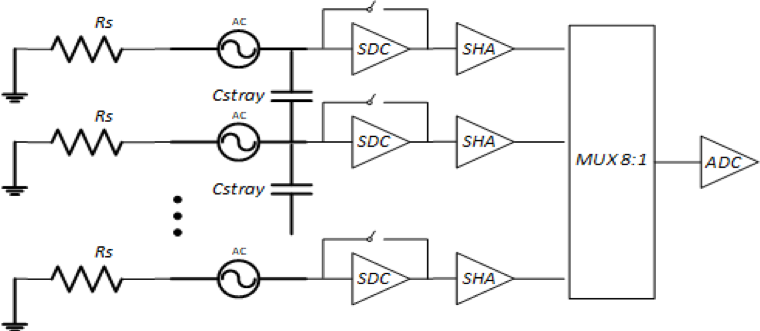
\includegraphics[width=0.7\linewidth]{figures/xtalk_schematic.png}
  \caption{Schematic diagram of the crosstalk measurement.}
  \label{fig:xtalk_schematic}
\end{figure}
\begin{figure}[h!]
\centering
  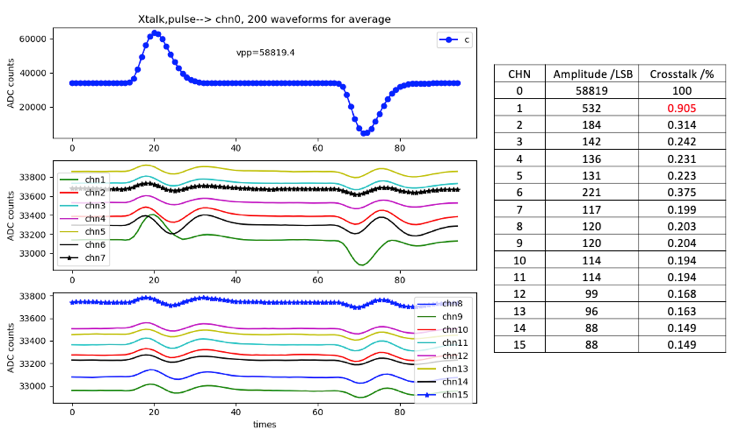
\includegraphics[width=0.7\linewidth]{figures/xtalk_RT.png}
  \caption{Crosstalk waveforms at room temperature. Calibration signal is injected in CHN0. The waveforms of the other 15 channels are shown in the bottom two plots. The amplitude of the cross talk is listed in the Table.}
  \label{fig:xtalk_RT}
\end{figure}
\begin{figure}[h!]
\centering
  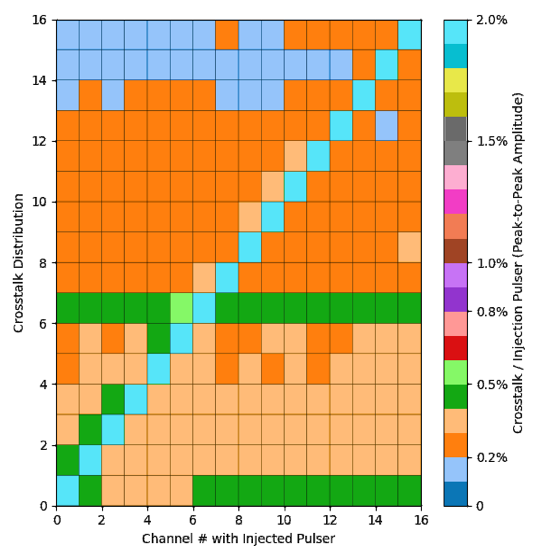
\includegraphics[width=0.7\linewidth]{figures/xtalk_LN2.png}
  \caption{Cross talk distribution at LN$_2$ temperature. The x-axis is the channel number with the injected pulse. The y-axis shows the amplitude of the crosstalk (in \%) for the remaining 15 channels.}
  \label{fig:xtalk_LN2}
\end{figure}

